\documentclass[]{report}
\usepackage{titlesec}
\usepackage{lipsum}
\usepackage{mathtools}
\usepackage{amsmath}
\usepackage{amssymb}
\usepackage{etoolbox}
\makeatletter
\patchcmd{\chapter}{\if@openright\cleardoublepage\else\clearpage\fi}{}{}{}
\makeatother



% Title Page
\title{Electrical and Computer Engineering \\
	Linear Programming (ECE 236A)\\
	Homework 1
	}
\author{Noyan Evirgen \\	
		205220656}

\titleformat{\chapter}[display]
{\normalfont\bfseries}{}{0pt}{\Large}
\begin{document}
\maketitle

\chapter{Problem 1}

First we need to define parameters for the problem. Let us assume that days of a week starting from Monday are numerated as $i = 1,2,...,5$ respectively. 
 
We have 2 constant vectors whose values can be defined as:
\begin{itemize}
	\item $b_i$ = Buying price defined for the $i$th day.
	\item $s_i$ = Selling price defined for the $i$th day.
\end{itemize}

We have 4 variables whose values can be defined as:
\begin{itemize}
	\item $m_i$ = Number of shares bought on $i$th day.
	\item $n_i$ = Number of shares sold on $i$th day.
	\item $x_i$ = Number of shares owned at the end of $i$th day.
	\item $y_i$ = Amount of money owned at the end of $i$th day. 
\end{itemize}

The objective is,
\begin{equation}
	max \{y_5\}
\end{equation}

such that,
\begin{equation}
\begin{split}
y_0 &= 100 \\
x_0 &= 0 \\
y_i &= y_{i-1} + s_i*n_i - b_i*m_i \\
x_i &= x_{i-1} + m_i - n_i \\
n_i & \leq x_{i-1} \\
b_i*m_i &\leq y_{i-1} \\
m_i, n_i, x_i, y_i &\geq 0
\end{split}
\end{equation}

Using the variables, the objective and the constraints, objective is optimized using cvxpy library (for the code see Appendix). The maximum amount of money one can have at the end of Friday is \$189.723. Optimal strategy is to buy shares on Tuesday with all the available money then sell all these shares on Wednesday. Next, shares are bought on Thursday with the entire available money and these shares are sold on Friday (for the results see Appendix).
 
\chapter{Problem 2} 

This optimization problem can not be expressed as an LP. Because, the optimization problem has strict inequality, 
\begin{equation}
	p_1 > p_i \quad \forall i \neq 1
\end{equation}
Strict inequalities can not be expressed in an LP.

\chapter{Problem 3}

Let us define $x_1$ as any point in the first hyperplane. We also define a line $L$ which passes through the point $x_1$ in the direction of $a$ which is the normal of the first hyperplane. Next, we define $x_2$ as the point where the line $L$ intersects with the second hyperplane. The distance between these two hyperplanes are equal to the distance between these two points. The equation of $L$ can be given by $x_1 + ak, \quad \forall k \in \mathbb{R}$. Since $x_2$ satisfies both the second hyperplane and $L$ equations, it can be found as follows,

\begin{equation}
	\begin{split}
	a^T&(x_1+ak) = b_2 \\
	k &= \frac{b_2-a^Tx_1}{a^Ta} \\
	k &= \frac{b_2-b_1}{a^Ta} \\
	\end{split}
\end{equation}
The intersection point $x_2$ can be found as,
\begin{equation}
	x_2 = x_1 + a\frac{b_2-b_1}{a^Ta}
\end{equation}
Therefore the distance between these hyperplanes are(which is equal to the distance between $x_1$ and $x_2$),
\begin{equation}
	\|x_1 - x_2\| = \frac{|b_1 - b_2|\|a\|}{a^Ta} = \frac{|b_1 - b_2|}{\|a\|}
\end{equation}

\chapter{Problem 4}

\section*{(a)}

The optimal solution is,

\[ x_i^* = \begin{cases} 
1, c_i &\leq 0 \\
0, c_i &> 0 
\end{cases}
\] 
and the optimal value is,

\[ p^* = \sum_{i=1}^{n}min(c_i,0)\]

\section*{(b)}

The optimal solution is,

\[ x_i^* = \begin{cases} 
1, c_i &\leq 0 \\
-1, c_i &> 0 
\end{cases}
\] 
and the optimal value is,

\[ p^* = -\sum_{i=1}^{n}|c_i|\]
\section*{(c)}

The optimal value is the summation of largest $k$ values. Let us define $s$ vector as the sorted vector whose values come from $c$ ($s_1 \geq s_2 \geq ... \geq s_n$). Then the optimal value is,

\[p^* = s_1 + s_2 + ... + s_k\]

The optimal solution has all the components zero except the ones that are in the first $k$ components of $s$. Their values are 1. In other words,

\[ x_i^* = \begin{cases} 
1, i \in A \\
0, i \notin A  
\end{cases}
\]

where $A$ is the set of the indices of $c$ with the largest $k$ values. 

\section*{(d)}

The optimal value is the sum of the largest $k$ positive components of $c$. If $c$ has less number of positive components than $k$, then the optimal solution is the summation of all of the positive components of $c$.

Let us define $s$ vector as the sorted vector whose values come from $c$ ($s_1 \geq s_2 \geq ... \geq s_n$). Then,

\begin{equation}
	t = max(i) \quad s.t. \quad( i \in 1,2,...,n \quad and \quad s_i \geq 0)
\end{equation}
Then the optimal value can be defined as,
\[p^* = s_1 + s_2 + ... + s_{min(t,k)}\]

Optimal solution,
\[ x_i^* = \begin{cases} 
1, i \in A \\
0, i \notin A  
\end{cases}
\]

where $A$ is the set of the indices of $c$ with the largest positive $min(t,k)$ values.

\section*{(e)}

In order to maximize $c^Tx$, we can also maximize $\alpha c^Tx$. Therefore, we maximize $(d^Tx)c^Tx$. The term in the parenthesis can be rewritten to make the entire term, $(x^Td)c^Tx$. This can be rewritten as $x^TAx$ where $A = dc^T$. The Lagrangian for this problem can be written as,

\begin{equation}
	\mathcal{L}(x) = x^TAx + \mu_1(x) + \mu_2(1-x)
\end{equation}
Taking the derivative and setting it to zero,
\begin{equation}
	x^T(A^T + A) = \mu_2 - \mu_1
\end{equation}
such that
\begin{equation}
\begin{split}
\mu_1(x) &= 0 \\
\mu_2(1-x) &= 0 \\
0 \leq x &\leq 1 \\
\mu_1, \mu_2 &\geq 0
\end{split}
\end{equation}

The equation can easily be solved to find the optimal solution and value. 

\appendix
\chapter{Appendix- Code for Problem 1}

Using the output of the code, the optimal strategy and the optimal value is given in Problem 1.

\begin{figure}
	\centering
	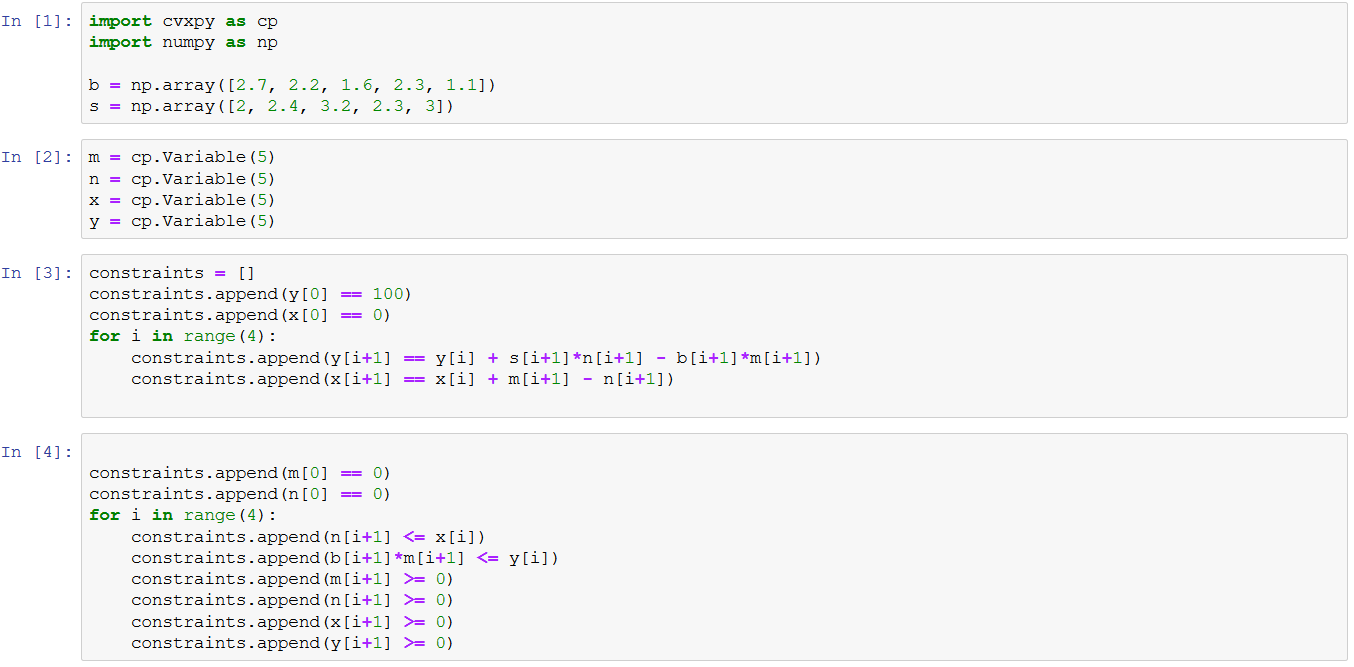
\includegraphics[width=1.2\linewidth]{code_1}
	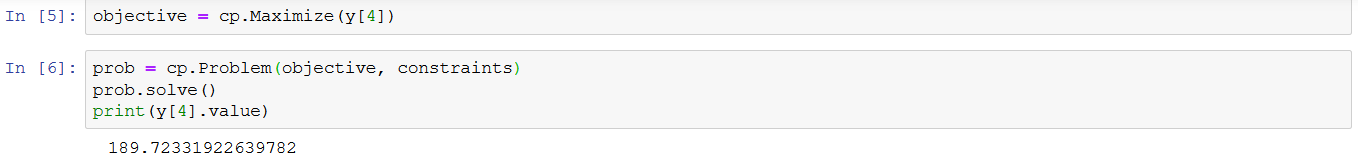
\includegraphics[width=1.2\linewidth]{code_2}
	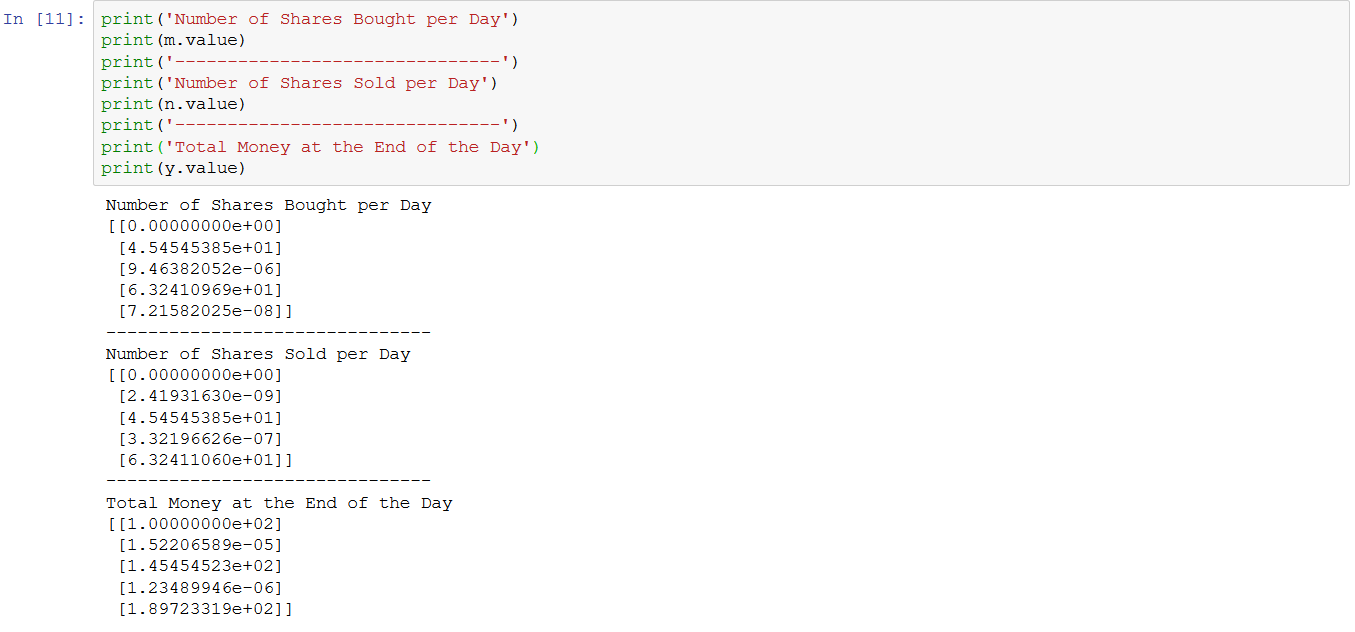
\includegraphics[width=1.2\linewidth]{code_3}
	\label{fig:code2}
\end{figure}

\end{document}          
